\appendix
\renewcommand{\thefigure}{\thesection\arabic{figure}}
\makeatletter
\@addtoreset{figure}{section}
\makeatother
\section{Pair entropy of chemical mixing in the liquid}
\label{app:entropy}

\begin{figure}[tbp]
    \centering
    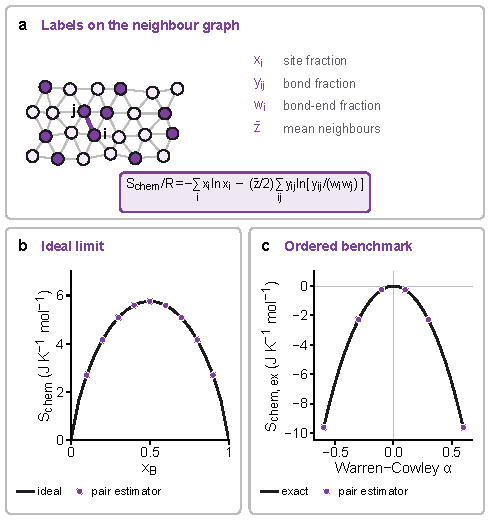
\includegraphics[width=83mm]{fig_pair_entropy_1col}
    \caption{The pair estimator of the chemical-mixing entropy and its tests, in \unit{\J\per\K\per\mole} of atoms. (a)~Schematic neighbor graph with the site, bond and bond-end fractions that enter the pair (quasi-chemical) estimator. (b)~Random labels on a lattice with $z = 12$: the pair estimator (circles) recovers the ideal entropy of mixing (line) to machine precision. (c)~Bethe lattice with $z = 12$ at $x_B = 0.5$: excess chemical entropy against the Warren--Cowley parameter, exact (line) and from the pair estimator (circles). The derivation awaits independent review.}
    \label{fig:pairentropy}
\end{figure}

In the method of Hong and Liu~\cite{hong2025entropy}, the entropy of a liquid simulated by molecular dynamics is separated into a vibrational part, obtained from the velocity autocorrelation function, and a configurational part that accounts for the arrangement of the chemical species. The configurational part can be expressed as the entropy of the species labels on the neighbor graph of the simulation, in which two atoms are connected when their distance is smaller than the first minimum of the corresponding partial radial distribution function (\cref{fig:pairentropy}a). Whatever the estimator, this entropy has a known limit. When the labels are distributed at random over the sites of the graph, it must reduce to the ideal entropy of mixing, $-R\sum_i x_i \ln x_i$, independently of the structure of the graph. In this work, the chemical-mixing term of Hong and Liu~\cite{hong2025entropy} is replaced with the pair approximation described below, which satisfies this limit exactly (\cref{fig:pairentropy}b).

In the pair (quasi-chemical) approximation~\cite{guggenheim1944mixtures,kikuchi1951cooperative}, the entropy per site of a lattice with coordination $z$ is obtained from the entropy of the bonds minus the entropy of the sites that each bond counts twice, $S/(N k_{\mathrm{B}}) = (z/2)\,H(y) - (z-1)\,H(x)$, where $H$ denotes the Shannon entropy, $x_i$ the fraction of species $i$ and $y_{ij}$ the fraction of bonds with $i$ at one end and $j$ at the other. For the neighbor graph of a liquid, in which the coordination varies from atom to atom, we write the same expression in terms of the mean coordination $\bar z$ and of the bond-end fractions $w_i = \sum_j y_{ij}$, which reduce to $x_i$ on a lattice:
\begin{equation}
\frac{S_{\mathrm{chem}}}{R} = -\sum_i x_i \ln x_i - \frac{\bar z}{2}\sum_{ij} y_{ij}\ln\frac{y_{ij}}{w_i w_j}.
\end{equation}
The second term is $-(\bar z/2)$ times the mutual information $I$ of the species at the two ends of a bond, so that the excess chemical entropy is $S^{\mathrm{ex}}_{\mathrm{chem}} = -R\,(\bar z/2)\,I$.

This form has three properties that make it suitable as an estimator. Since $I = 0$ for random labels on any graph, the entropy reduces exactly to the ideal entropy of mixing in this limit, and since $I \ge 0$, any chemical order, whether ordering or clustering, lowers the entropy. In addition, the expression is exact for the quasi-chemical distribution on a Bethe lattice and for a one-dimensional chain, and it remains an approximation in other cases. The estimator was tested by permuting the species labels on the neighbor graphs of the Cr--Ni simulations, which gives excess chemical entropies of the order of $10^{-3}$~\unit{\J\per\K\per\mole} (\cref{fig:entropy}b), and on ordered benchmarks with Warren--Cowley parameters between $-0.6$ and $0.6$, for which it reproduces the exact excess entropy of the Bethe lattice (\cref{fig:pairentropy}c). The effect of the neighbor cutoff is included in the uncertainty of the estimate. Until the derivation has been reviewed independently, the excess entropies obtained with this estimator are treated as provisional. The estimator and its tests are available in the package \texttt{pair-entropy}~\cite{pairentropy}.


\section{Assessment trajectory and calculated phase states}
\label{app:assessment}

The assessment dashboard records how the candidate solutions change during
the fitting sequence and where the selected fit lies in parameter space. To
make its four views readable at column width, we show them separately in
\cref{fig:dashboard-objective,fig:dashboard-optimizer,fig:dashboard-parameters,fig:dashboard-projection}.
Panel (a) gives the negative log posterior for each start; because evidence is
added at each step, these values are comparable only within a step. Panel (b)
follows the eight starts of step 4c-b against the topology criterion. Panel
(c) shows how the 14 parameters change along the selected lineage, scaled by
their prior standard deviations, while panel (d) projects the starts, lineage,
and Laplace-mixture draws onto the dashboard's fixed PCA coordinates.

\begin{figure}[tbp]
    \centering
    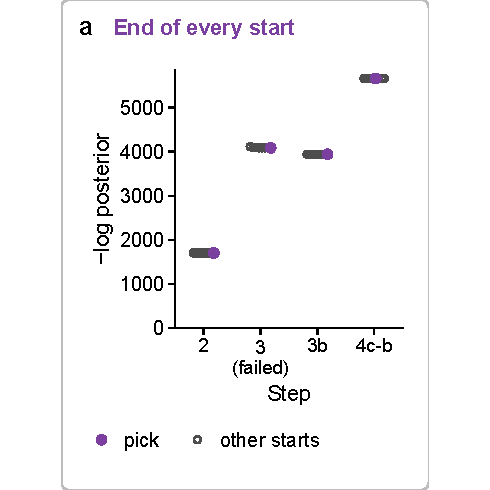
\includegraphics[width=83mm]{fig_crni_dashboard_panel_a}
    \caption{Negative log posterior at the end of each start in steps 2, 3,
    3b, and 4c-b; the selected start is purple. Objective values across steps
    are comparable only within each step because the evidence changes.}
    \label{fig:dashboard-objective}
\end{figure}

\begin{figure}[tbp]
    \centering
    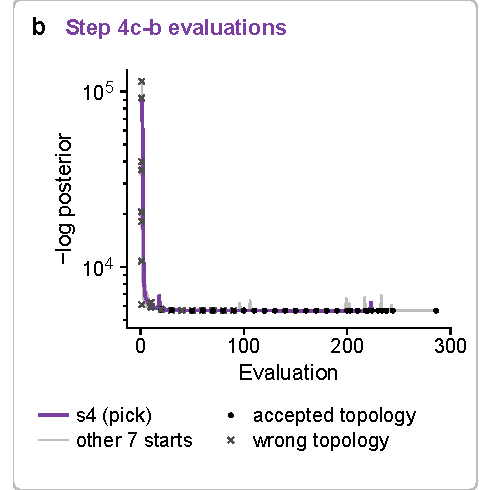
\includegraphics[width=83mm]{fig_crni_dashboard_panel_b}
    \caption{Evaluations of the eight step-4c-b starts; topology was
    classified every 10 evaluations.}
    \label{fig:dashboard-optimizer}
\end{figure}

\begin{figure}[tbp]
    \centering
    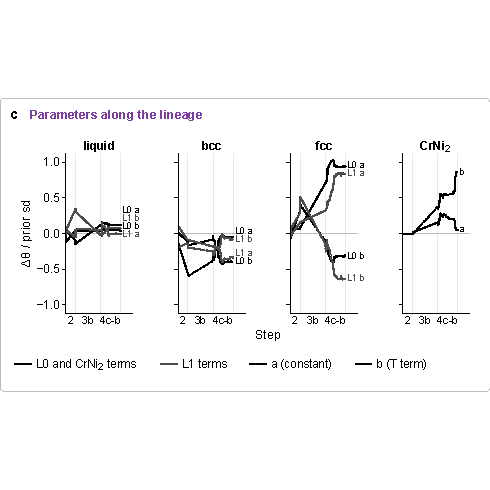
\includegraphics[width=83mm]{fig_crni_dashboard_panel_c}
    \caption{Changes in the 14 parameters along the selected lineage, in
    units of the prior standard deviation.}
    \label{fig:dashboard-parameters}
\end{figure}

\begin{figure}[tbp]
    \centering
    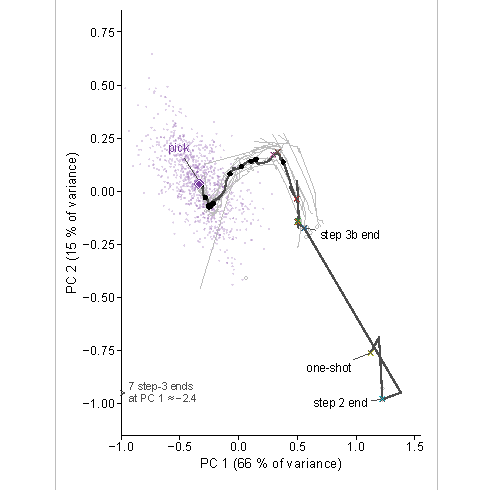
\includegraphics[width=83mm]{fig_crni_dashboard_panel_d}
    \caption{Projection of starts, lineage, and uncertainty samples onto the
    fixed PCA basis used by the dashboard. The purple points are 1,000
    Laplace-mixture draws and the purple diamonds are the mode centres. The
    dark line traces the selected lineage, black dots mark accepted topology,
    and crosses mark topology violations. Grey lines show the other step-4c-b
    starts, and open circles show the other starts. Seven
    failed step-3 endpoints lie outside the plotted range, at a mean PC 1 of
    approximately $-2.4$.}
    \label{fig:dashboard-projection}
\end{figure}

The one-shot calculation provides the starting description for the refinement
discussed in the main text. In \cref{fig:oneshot}, panel (a) shows the
PhaseForge model before adding the excess entropy of the liquid, and panel (b)
shows the change after it is included. The Lee assessment \cite{lee1992} and
observations compiled in ORCHID provide a reference for both calculations.
The markers distinguish phase assemblages from transition temperatures, and
experimental transition temperatures from values reported by models. This
comparison shows what the liquid entropy changes before the remaining
differences are addressed by fitting.

\begin{figure}[tbp]
    \centering
    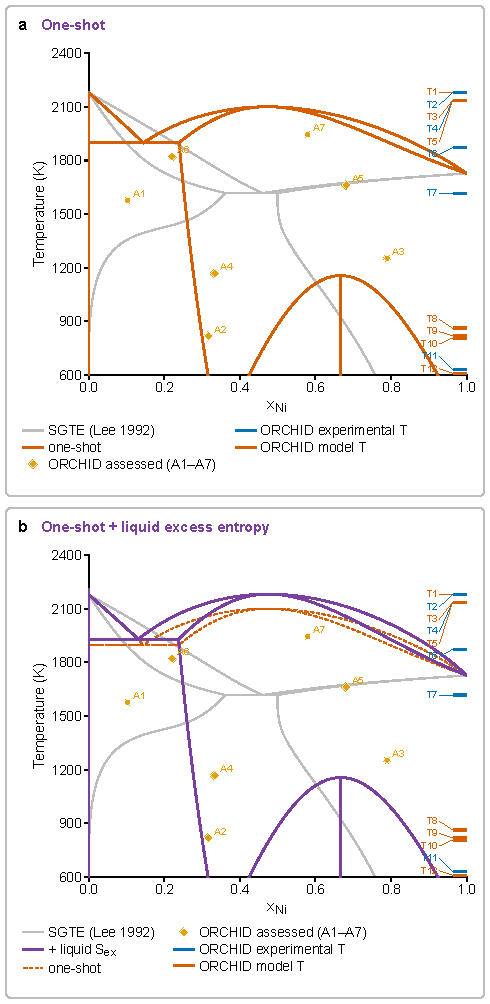
\includegraphics[width=83mm]{fig_crni_oneshot_1col_orchid}
    \caption{Phase diagram of the PhaseForge one-shot model of Cr--Ni,
    calculated with pycalphad, (a) without and (b) with the excess entropy of
    the liquid. Orange lines show the one-shot model and purple lines show the
    model with the liquid excess entropy; orange dashed lines in (b) reproduce
    panel (a). Light grey lines show the assessment of Lee
    \cite{lee1992}. Orange markers (A1--A7) denote assessed assemblages in
    ORCHID, with circles for single-phase fields and diamonds for two-phase
    fields. Marks at the right edge (T1--T12) denote transition and invariant
    temperatures without an assigned composition; blue marks are experimental
    and orange-red marks are model values. Records naming Al--Cr--Ni phases are
    excluded. The plotted observations are from ORCHID v2026.10 and the sources
    cited in the main text.}
    \label{fig:oneshot}
\end{figure}

We checked the final assessment at 695 observed states, comprising 329
phase-boundary records and 366 states with information about phases absent
at equilibrium. At each reported temperature and composition, we calculated
the stable assemblage at 101325 Pa and compared it with the observed phases.
A partial tie line reports one end of an equilibrium, leaving the composition
of the coexisting phase unspecified. As shown in
\cref{fig:state-match-summary}, the calculated assemblage contains all
observed phases at 599 states, while exact agreement occurs at 424. These
measures differ because inclusion allows the calculation to predict
additional phases. The comparison is made at the reported coordinates and
does not account for measurement uncertainty; the main text discusses how
this affects its interpretation.

\begin{figure}[tbp]
    \centering
    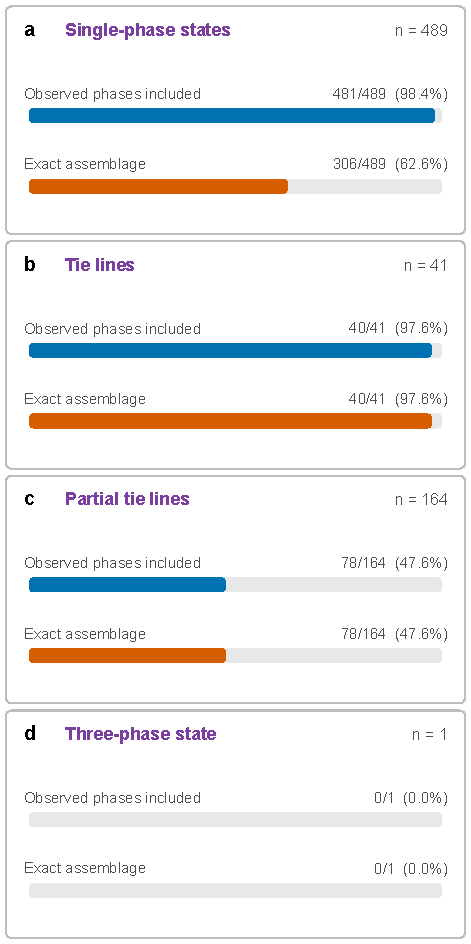
\includegraphics[width=83mm]{fig_state_comparison_1col}
    \caption{Comparison of calculated and observed phase assemblages by
    evidence type for the 695 states. Blue bars show the fraction for which
    all observed phases occur in the calculated assemblage; orange bars show
    exact assemblage agreement. Counts and percentages are given at right.}
    \label{fig:state-match-summary}
\end{figure}
